\documentclass[12pt]{article}

\usepackage[a4paper,margin=1in]{geometry}
\usepackage{amsmath,amssymb}
\usepackage{newtxtext,newtxmath} % Times-style font
\usepackage{fancyhdr}
\usepackage{listings}
\usepackage{graphicx}
\usepackage{float}
\usepackage{algorithm}
\usepackage{algpseudocode}
\usepackage{booktabs}
\usepackage{xcolor}

\setlength{\textfloatsep}{10pt}
\setlength{\floatsep}{10pt}

\setlength{\parindent}{0pt}
\setlength{\parskip}{5pt}

% Keep entire document at 12 pt
\AtBeginDocument{
    \fontsize{12pt}{14pt}\selectfont
}

\lstdefinestyle{code}{
    language=Python,
    basicstyle=\ttfamily\fontsize{9.5pt}{11.5pt}\selectfont,
    breaklines=true,
    breakatwhitespace=false,
    frame=single,
    numbers=left,
    numberstyle=\tiny\color{gray},
    keywordstyle=\color{blue},
    commentstyle=\color{gray},
    stringstyle=\color{green!50!black},
    columns=fullflexible,
    keepspaces=true,
    showstringspaces=false
}

\lstdefinestyle{output}{
    basicstyle=\ttfamily\fontsize{9pt}{11pt}\selectfont,
    breaklines=true,
    breakatwhitespace=false,
    frame=single,
    numbers=none,
    backgroundcolor=\color{gray!6},
    columns=fullflexible,
    keepspaces=true,
    showstringspaces=false
}

% ------------------------------------------------
% Header
% ------------------------------------------------

\pagestyle{fancy}
\fancyhf{}

\fancyhead[L]{Name: Kishan Sahu{\hspace{4cm}}}
\fancyhead[R]{Enrollment No.: P26DS017{\hspace{3.5cm}}}

\renewcommand{\headrulewidth}{0.4pt}
\setlength{\headheight}{15pt}

% ------------------------------------------------
% Code formatting
% ------------------------------------------------

\lstset{
    basicstyle=\ttfamily\fontsize{9.5pt}{11.5pt}\selectfont,
    breaklines=true,
    frame=single,
    columns=fullflexible,
    keepspaces=true,
    showstringspaces=false
}

\begin{document}

% ------------------------------------------------
% TITLE
% ------------------------------------------------

\begin{center}
\textbf{Computer Science and Engineering Department, SVNIT, Surat}\\
\textbf{M.Tech. I -- Semester I}\\
\textbf{Machine Learning (CSDS105)}\\
\textbf{Lab Assignment 8: Support Vector Machines (SVM) for Text Classification and Non-Linear Kernel Exploration}
\end{center}

\vspace{0.3cm}

\section{Introduction and Problem Formulation}

Text classification presents unique computational and statistical challenges due to extreme feature dimensionality, severe sparsity ($>99\%$), and acute class imbalance. Traditional linear models often suffer from overfitting or boundary instability when the number of features exceeds the number of informative training instances. To address these vulnerabilities, \textbf{Support Vector Machines (SVM)}, pioneered by Vladimir Vapnik (1995), formulate classification as a convex quadratic programming optimization problem grounded in \textbf{Structural Risk Minimization (SRM)}.

Unlike empirical risk minimization algorithms that seek any separating hyperplane that minimizes training error (e.g., Perceptrons or unregularized logistic models), SVM discovers the unique \textbf{Maximum-Margin Hyperplane} that maximizes the geometric distance to the closest training exemplars (the \textit{support vectors}). 

This laboratory assignment conducts an empirical study on the canonical Kaggle SMS Spam dataset ($N=5,572$ instances), executing two core investigations:
\begin{enumerate}
    \item \textbf{Primary Algorithm Benchmark}: Benchmarking Linear Support Vector Classification against two distinct learning paradigms: an eager recursive tree partitioner (\textbf{Decision Tree}) and an instance-based lazy learner (\textbf{K-Nearest Neighbors} equipped with Cosine distance).
    \item \textbf{Non-Linear Kernel & Scaling Exploration}: Evaluating non-linear mapping transformations across four distinct kernel methods (\textbf{Linear}, \textbf{Radial Basis Function [RBF]}, \textbf{Polynomial}, and \textbf{Sigmoid}) under both unscaled and \textbf{MaxAbsScaler} normalized Term Frequency-Inverse Document Frequency (TF-IDF) feature representations.
\end{enumerate}

\subsection{Dataset Overview and Exploratory Inspection}
The corpus comprises $N = 5,572$ mobile messages categorized as legitimate (\texttt{ham}) or spam (\texttt{spam}). Table~\ref{tab:dataset_dist} details the target distribution.

\begin{table}[H]
\centering
\caption{Target Class Distribution of the SMS Spam Dataset}
\label{tab:dataset_dist}
\vspace{0.2cm}
\begin{tabular}{lccc}
\toprule
\textbf{Class Label} & \textbf{Encoded Target} & \textbf{Instance Count} & \textbf{Percentage (\%)} \\
\midrule
Ham (Legitimate) & 0 & 4,825 & 86.59\% \\
Spam (Fraudulent) & 1 & 747 & 13.41\% \\
\midrule
\textbf{Total} & -- & \textbf{5,572} & \textbf{100.00\%} \\
\bottomrule
\end{tabular}
\end{table}

The severe class imbalance ($86.59\%$ vs. $13.41\%$) requires stratified partitioning and comprehensive evaluation spanning Precision, Recall, and the balanced F1-Score rather than naive overall accuracy.

\newpage
\section{Mathematical Foundations of Support Vector Machines}

\subsection{The Maximum-Margin Hyperplane (Hard-Margin Formulation)}
Consider a linearly separable binary classification dataset $\mathcal{D} = \{(\mathbf{x}_i, y_i)\}_{i=1}^N$, where $\mathbf{x}_i \in \mathbb{R}^D$ and $y_i \in \{-1, +1\}$. A linear decision surface is defined by weight vector $\mathbf{w} \in \mathbb{R}^D$ and bias scalar $b \in \mathbb{R}$:
\begin{equation}
    f(\mathbf{x}) = \mathbf{w}^T \mathbf{x} + b = 0
\end{equation}
The geometric distance from an arbitrary point $\mathbf{x}_i$ to the hyperplane is:
\begin{equation}
    \gamma_i = \frac{y_i (\mathbf{w}^T \mathbf{x}_i + b)}{\|\mathbf{w}\|_2}
\end{equation}
The optimal separating hyperplane maximizes the margin $\gamma = \min_i \gamma_i$. Rescaling $\mathbf{w}$ and $b$ such that the closest support vectors satisfy $y_i(\mathbf{w}^T \mathbf{x}_i + b) = 1$, the margin becomes $\frac{1}{\|\mathbf{w}\|}$. Maximizing $\frac{1}{\|\mathbf{w}\|}$ is mathematically equivalent to minimizing $\frac{1}{2}\|\mathbf{w}\|^2$:
\begin{equation}
    \min_{\mathbf{w}, b} \frac{1}{2} \|\mathbf{w}\|^2 \quad \text{subject to } y_i(\mathbf{w}^T \mathbf{x}_i + b) \ge 1, \quad \forall i = 1, \dots, N
\end{equation}

\subsection{Soft-Margin Formulation and Slack Variables}
Real-world text feature spaces contain noise, linguistic ambiguity, and overlapping tokens, precluding strict linear separability. Cortes and Vapnik (1995) introduced non-negative slack variables $\xi_i \ge 0$ allowing margin violations, penalized by regularization hyperparameter $C > 0$:
\begin{equation}
    \min_{\mathbf{w}, b, \boldsymbol{\xi}} \frac{1}{2} \|\mathbf{w}\|^2 + C \sum_{i=1}^{N} \xi_i \quad \text{s.t. } y_i(\mathbf{w}^T \mathbf{x}_i + b) \ge 1 - \xi_i, \quad \xi_i \ge 0, \quad \forall i
\end{equation}
The hyperparameter $C$ governs the bias-variance trade-off:
\begin{itemize}
    \item \textbf{Large $C$}: Heavily penalizes misclassifications, leading to a narrower margin and risking overfitting.
    \item \textbf{Small $C$}: Encourages a wider margin at the expense of tolerating training classification errors.
\end{itemize}

\subsection{Wolfe Dual Formulation}
Applying Lagrangian duality with multipliers $\alpha_i \ge 0$ and $\mu_i \ge 0$, the primal problem transforms into its Wolfe dual representation:
\begin{equation}
    \max_{\boldsymbol{\alpha}} \sum_{i=1}^{N} \alpha_i - \frac{1}{2} \sum_{i=1}^{N} \sum_{j=1}^{N} \alpha_i \alpha_j y_i y_j (\mathbf{x}_i^T \mathbf{x}_j) \quad \text{s.t. } 0 \le \alpha_i \le C, \quad \sum_{i=1}^{N} \alpha_i y_i = 0
\end{equation}
The optimal weight vector is an explicit linear combination of the support vectors ($\alpha_i > 0$):
\begin{equation}
    \mathbf{w}^* = \sum_{i=1}^{N} \alpha_i^* y_i \mathbf{x}_i = \sum_{i \in \text{SV}} \alpha_i^* y_i \mathbf{x}_i
\end{equation}

\subsection{The Kernel Trick and Mercer's Theorem}
A profound advantage of the dual formulation is that input features $\mathbf{x}_i, \mathbf{x}_j$ appear exclusively through their pairwise inner product $\mathbf{x}_i^T \mathbf{x}_j$. If the data is non-linearly separable in input space $\mathbb{R}^D$, it can be mapped into a higher (potentially infinite) dimensional Hilbert space $\mathcal{H}$ via non-linear mapping $\Phi(\mathbf{x})$.

By \textbf{Mercer's Theorem}, any continuous symmetric positive semi-definite function $K(\mathbf{x}_i, \mathbf{x}_j)$ directly computes this inner product without explicitly constructing $\Phi(\mathbf{x})$:
\begin{equation}
    K(\mathbf{x}_i, \mathbf{x}_j) = \langle \Phi(\mathbf{x}_i), \Phi(\mathbf{x}_j) \rangle_{\mathcal{H}}
\end{equation}

The four kernel functions evaluated in this study are:
\begin{enumerate}
    \item \textbf{Linear Kernel}:
    \begin{equation}
        K_{\text{Linear}}(\mathbf{x}_i, \mathbf{x}_j) = \mathbf{x}_i^T \mathbf{x}_j
    \end{equation}
    \item \textbf{Radial Basis Function (RBF / Gaussian) Kernel}:
    \begin{equation}
        K_{\text{RBF}}(\mathbf{x}_i, \mathbf{x}_j) = \exp\left( -\gamma \|\mathbf{x}_i - \mathbf{x}_j\|^2 \right) \quad (\gamma = \frac{1}{D \cdot \sigma^2})
    \end{equation}
    \item \textbf{Polynomial Kernel}:
    \begin{equation}
        K_{\text{Poly}}(\mathbf{x}_i, \mathbf{x}_j) = (\gamma \mathbf{x}_i^T \mathbf{x}_j + r)^d \quad (d=3, r=0)
    \end{equation}
    \item \textbf{Sigmoid (Hyperbolic Tangent) Kernel}:
    \begin{equation}
        K_{\text{Sigmoid}}(\mathbf{x}_i, \mathbf{x}_j) = \tanh\left( \gamma \mathbf{x}_i^T \mathbf{x}_j + r \right)
    \end{equation}
\end{enumerate}

\newpage
\section{Text Preprocessing and Feature Extraction}

\subsection{Environment Configuration and Data Loading}
The implementation utilizes Scikit-Learn's estimators (`SVC`, `DecisionTreeClassifier`, `KNeighborsClassifier`), `TfidfVectorizer`, and `MaxAbsScaler`.

\begin{lstlisting}[style=code]
import os
import warnings
warnings.filterwarnings("ignore")

import numpy as np
import pandas as pd
import matplotlib.pyplot as plt
import seaborn as sns

from sklearn.model_selection import train_test_split
from sklearn.feature_extraction.text import TfidfVectorizer
from sklearn.preprocessing import MaxAbsScaler
from sklearn.svm import SVC
from sklearn.tree import DecisionTreeClassifier
from sklearn.neighbors import KNeighborsClassifier
from sklearn.metrics import (
    accuracy_score, precision_score, recall_score, f1_score,
    classification_report, confusion_matrix, ConfusionMatrixDisplay
)
\end{lstlisting}

\subsection{Sublinear TF-IDF Vectorization}
Raw text is tokenized, stripped of standard English stopwords, and mapped to a maximum vocabulary of $D = 2,500$ terms using \textbf{Sublinear Term Frequency} scaling:
\begin{align}
    \text{TF}_{\text{sublinear}}(t, d) &= 1 + \ln(\text{count}(t, d)) \quad \text{for } \text{count} > 0 \\
    \text{IDF}(t, \mathcal{D}) &= \ln\left( \frac{1 + N}{1 + \text{DF}(t)} \right) + 1 \\
    \text{TF-IDF}(t, d) &= \text{TF}_{\text{sublinear}}(t, d) \times \text{IDF}(t, \mathcal{D})
\end{align}
Rows are normalized to unit Euclidean length ($\|\mathbf{x}_i\|_2 = 1.0$), eliminating document length bias.

\begin{lstlisting}[style=code]
X = df["text"]
y = df["target"]

# Stratified 80/20 train/test split to preserve class imbalance
X_train, X_test, y_train, y_test = train_test_split(
    X, y, test_size=0.20, random_state=42, stratify=y
)

# Fit TF-IDF Vectorizer on training data only
tfidf = TfidfVectorizer(
    max_features=2500,
    stop_words="english",
    sublinear_tf=True
)

X_train_tfidf = tfidf.fit_transform(X_train)
X_test_tfidf = tfidf.transform(X_test)

sparsity = 100.0 * (1.0 - (X_train_tfidf.nnz / (X_train_tfidf.shape[0] * X_train_tfidf.shape[1])))
print(f"Training set shape: {X_train_tfidf.shape[0]} samples, {X_train_tfidf.shape[1]} vocabulary features")
print(f"Testing set shape:  {X_test_tfidf.shape[0]} samples, {X_test_tfidf.shape[1]} vocabulary features")
print(f"Sparsity: {sparsity:.2f}% zero entries")
\end{lstlisting}

\begin{lstlisting}[style=output]
Training set shape: 4457 samples, 2500 vocabulary features
Testing set shape:  1115 samples, 2500 vocabulary features
Sparsity: 99.74% zero entries
\end{lstlisting}

\subsection{Feature Scaling: MaxAbsScaler}
Standard $Z$-score scaling (`StandardScaler`) subtracts empirical means, converting sparse matrices into dense memory-prohibitive matrices and destroying the sparse structural integrity of text. Instead, \textbf{MaxAbsScaler} scales each feature by its maximum absolute value without centering:
\begin{equation}
    x_{ij}' = \frac{x_{ij}}{\max_k |x_{kj}|} \in [0, 1]
\end{equation}
This scales sparse TF-IDF features to $[0, 1]$ while strictly preserving exact matrix sparsity ($99.74\%$).

\newpage
\section{Primary Algorithm Benchmarking: Linear SVM vs. Decision Tree vs. KNN}

\subsection{Model Setup and Evaluation}
Linear SVM ($C=1.0$), Decision Tree ($\text{max\_depth}=20$), and KNN ($k=5$ with Cosine metric) are fitted on the training partition ($N=4,457$) and evaluated on testing instances ($N=1,115$).

\begin{lstlisting}[style=code]
benchmark_models = {
    "Linear SVM": SVC(kernel="linear", C=1.0, random_state=42),
    "Decision Tree": DecisionTreeClassifier(max_depth=20, random_state=42),
    "KNN (Cosine)": KNeighborsClassifier(n_neighbors=5, metric="cosine")
}

algo_results = []
algo_predictions = {}

for name, model in benchmark_models.items():
    model.fit(X_train_tfidf, y_train)
    y_pred = model.predict(X_test_tfidf)
    algo_predictions[name] = y_pred
    
    algo_results.append({
        "Algorithm": name,
        "Accuracy": round(accuracy_score(y_test, y_pred), 4),
        "Precision": round(precision_score(y_test, y_pred), 4),
        "Recall": round(recall_score(y_test, y_pred), 4),
        "F1-Score": round(f1_score(y_test, y_pred), 4)
    })

algo_df = pd.DataFrame(algo_results)
\end{lstlisting}

\begin{lstlisting}[style=output]
=== Algorithm Comparison Summary ===
    Algorithm  Accuracy  Precision  Recall  F1-Score
   Linear SVM    0.9821     0.9924  0.8725    0.9286
Decision Tree    0.9534     0.8489  0.7919    0.8194
 KNN (Cosine)    0.9668     0.9667  0.7785    0.8625
\end{lstlisting}

\subsection{Quantitative Results and Classification Reports}
Table~\ref{tab:algo_results} compares quantitative test performance across all three primary models.

\begin{table}[H]
\centering
\caption{Performance Comparison of Linear SVM, Decision Tree, and KNN}
\label{tab:algo_results}
\vspace{0.2cm}
\begin{tabular}{lcccc}
\toprule
\textbf{Classification Algorithm} & \textbf{Accuracy} & \textbf{Precision (Spam)} & \textbf{Recall (Spam)} & \textbf{F1-Score (Spam)} \\
\midrule
\textbf{Linear SVM}  & \textbf{0.9821 (98.21\%)} & \textbf{0.9924} & \textbf{0.8725} & \textbf{0.9286} \\
Decision Tree        & 0.9534 (95.34\%)          & 0.8489          & 0.7919          & 0.8194          \\
KNN (Cosine Metric)  & 0.9668 (96.68\%)          & 0.9667          & 0.7785          & 0.8625          \\
\bottomrule
\end{tabular}
\end{table}

\begin{lstlisting}[style=output]
=======================================================
Detailed Classification Reports
=======================================================
>>> Linear SVM <<<
              precision    recall  f1-score   support
     Ham (0)       0.98      1.00      0.99       966
    Spam (1)       0.99      0.87      0.93       149
    accuracy                           0.98      1115

>>> Decision Tree <<<
              precision    recall  f1-score   support
     Ham (0)       0.97      0.98      0.97       966
    Spam (1)       0.85      0.79      0.82       149
    accuracy                           0.95      1115

>>> KNN (Cosine) <<<
              precision    recall  f1-score   support
     Ham (0)       0.97      1.00      0.98       966
    Spam (1)       0.97      0.78      0.86       149
    accuracy                           0.97      1115
\end{lstlisting}

\subsection{Visual Diagnostic Comparison}
Figure~\ref{fig:algo_bars} contrasts the performance metrics, and Figure~\ref{fig:algo_cm} illustrates the confusion matrix heatmaps. Linear SVM produced only $1$ False Positive out of $966$ legitimate messages ($99.24\%$ precision) while correctly capturing $130$ spam messages ($87.25\%$ recall).

\begin{figure}[H]
    \centering
    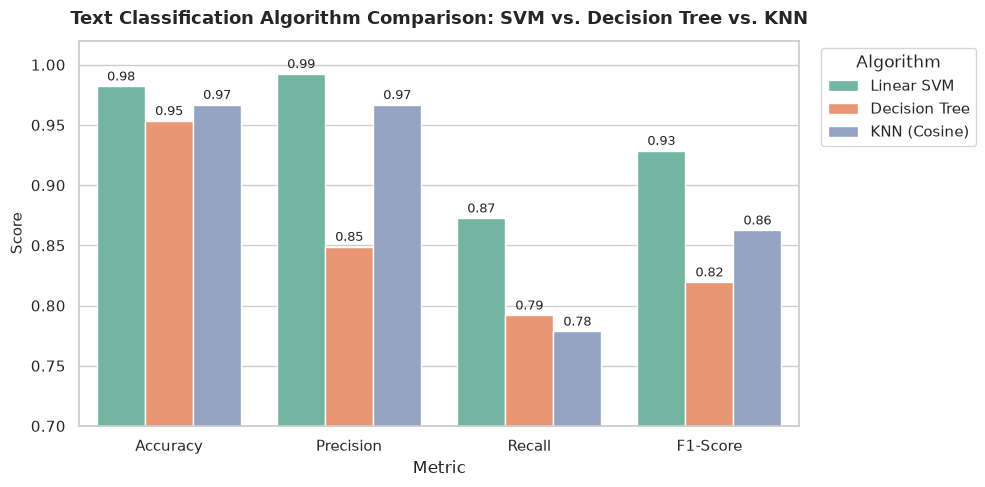
\includegraphics[width=0.78\textwidth]{figures/svm_algo_comparison_bars.png}
    \caption{Comparative performance metrics (Accuracy, Precision, Recall, and F1-Score) across Linear SVM, Decision Tree, and KNN (Cosine).}
    \label{fig:algo_bars}
\end{figure}

\begin{figure}[H]
    \centering
    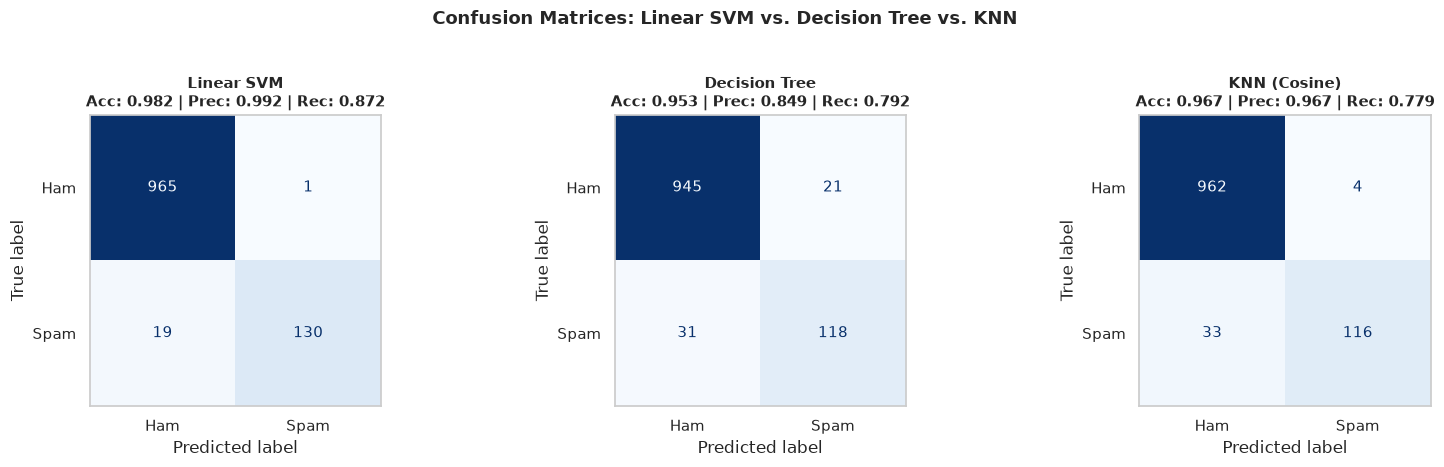
\includegraphics[width=0.98\textwidth]{figures/svm_primary_algos_cm.png}
    \caption{Confusion matrix heatmaps for Linear SVM, Decision Tree, and KNN (Cosine) on test samples ($N=1,115$).}
    \label{fig:algo_cm}
\end{figure}

\newpage
\section{Kernel Methods Exploration and Feature Scaling Effects}

\subsection{Kernel Benchmarking Protocol}
To evaluate non-linear hypothesis spaces, four kernel functions are fitted across both unscaled and MaxAbs scaled TF-IDF matrices:
\begin{equation}
    \text{Kernels} \in \{\text{Linear}, \text{RBF}, \text{Polynomial } (d=3), \text{Sigmoid}\}
\end{equation}

\begin{lstlisting}[style=code]
scaler = MaxAbsScaler()
X_train_scaled = scaler.fit_transform(X_train_tfidf)
X_test_scaled = scaler.transform(X_test_tfidf)

kernels = ["linear", "rbf", "poly", "sigmoid"]
kernel_results = []
kernel_predictions = {}

for scaling_name, tr_data, te_data in [
    ("Unscaled TF-IDF", X_train_tfidf, X_test_tfidf),
    ("MaxAbs Scaled", X_train_scaled, X_test_scaled)
]:
    for k in kernels:
        svm = SVC(kernel=k, C=1.0, random_state=42)
        svm.fit(tr_data, y_train)
        y_pred = svm.predict(te_data)
        
        kernel_name = f"{k.capitalize()} ({scaling_name})"
        kernel_predictions[kernel_name] = y_pred
        
        kernel_results.append({
            "Kernel": k.capitalize(),
            "Scaling": scaling_name,
            "Accuracy": round(accuracy_score(y_test, y_pred), 4),
            "Precision": round(precision_score(y_test, y_pred), 4),
            "Recall": round(recall_score(y_test, y_pred), 4),
            "F1-Score": round(f1_score(y_test, y_pred), 4)
        })

kernel_df = pd.DataFrame(kernel_results)
\end{lstlisting}

\subsection{Kernel and Scaling Performance Synthesis}
Table~\ref{tab:kernel_results} synthesizes the empirical performance across all eight kernel and scaling configurations.

\begin{table}[H]
\centering
\caption{Comprehensive Performance Breakdown Across SVM Kernels and Feature Scaling}
\label{tab:kernel_results}
\vspace{0.2cm}
\begin{tabular}{llcccc}
\toprule
\textbf{Kernel Function} & \textbf{Feature Scaling} & \textbf{Accuracy} & \textbf{Precision} & \textbf{Recall} & \textbf{F1-Score} \\
\midrule
\textbf{Linear}  & \textbf{Unscaled TF-IDF} & \textbf{0.9821} & 0.9924 & 0.8725 & \textbf{0.9286} \\
RBF              & Unscaled TF-IDF          & 0.9803          & \textbf{1.0000} & 0.8523 & 0.9203 \\
Polynomial ($d=3$) & Unscaled TF-IDF        & 0.9453          & \textbf{1.0000} & 0.5906 & 0.7426 \\
Sigmoid          & Unscaled TF-IDF          & 0.9803          & 0.9847 & 0.8658 & 0.9214 \\
\midrule
Linear           & MaxAbs Scaled            & 0.9812          & 0.9706 & \textbf{0.8859} & 0.9263 \\
RBF              & MaxAbs Scaled            & 0.9731          & 0.9161 & 0.8792 & 0.8973 \\
Polynomial ($d=3$) & MaxAbs Scaled          & 0.9462          & \textbf{1.0000} & 0.5973 & 0.7479 \\
Sigmoid          & MaxAbs Scaled            & 0.9803          & 0.9704 & 0.8792 & 0.9225 \\
\bottomrule
\end{tabular}
\end{table}

\subsection{Kernel Visual Diagnostics}
Figure~\ref{fig:kernel_bars} illustrates F1-scores across scaling regimes, and Figure~\ref{fig:kernel_cm} shows confusion matrices for all four kernels under unscaled TF-IDF.

\begin{figure}[H]
    \centering
    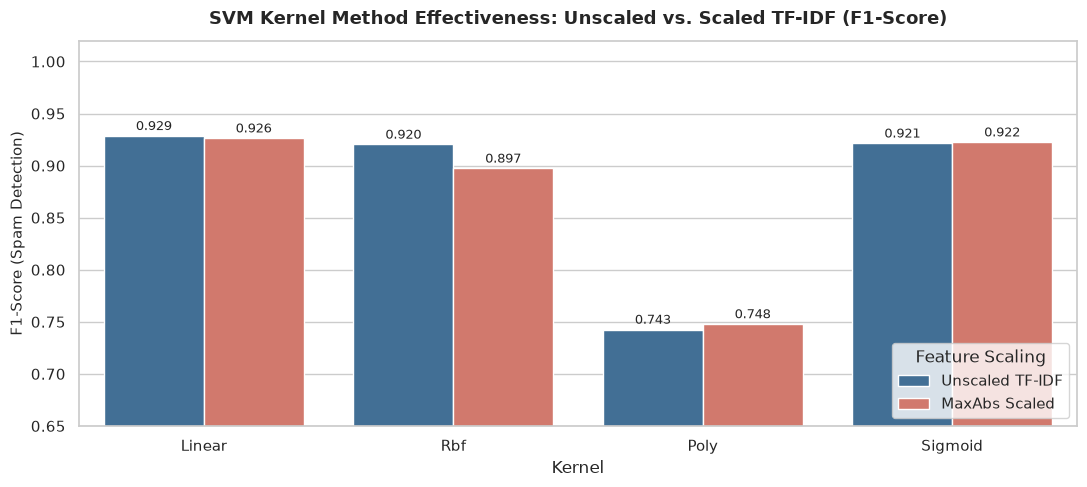
\includegraphics[width=0.82\textwidth]{figures/svm_kernel_scaling_bars.png}
    \caption{SVM Kernel Method F1-Score comparison under Unscaled vs. MaxAbs Scaled TF-IDF representations.}
    \label{fig:kernel_bars}
\end{figure}

\begin{figure}[H]
    \centering
    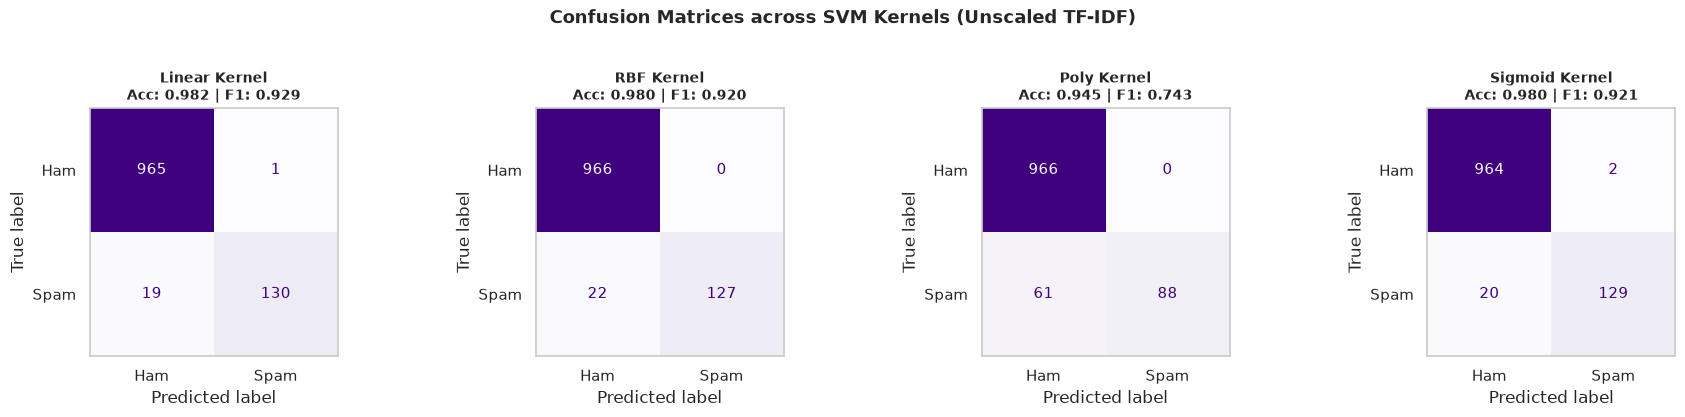
\includegraphics[width=0.98\textwidth]{figures/svm_kernels_cm.png}
    \caption{Confusion matrix heatmaps for Linear, RBF, Polynomial, and Sigmoid kernels on test samples ($N=1,115$).}
    \label{fig:kernel_cm}
\end{figure}

\newpage
\section{In-Depth Discussion: High-Dimensional Text Geometry}

The empirical benchmarks reveal profound geometric insights governing SVM behavior in textual NLP domains:

\subsection{1. Why Linear SVM Dominates Text Classification}
Text classification operates in ultra-high dimensional sparse spaces ($D = 2,500$ vocabulary dimensions with $99.74\%$ sparsity). Under high dimensionality:
\begin{itemize}
    \item \textbf{Quasi-Linear Separability}: By Cover's Theorem on the separability of patterns, randomly assigned patterns in high-dimensional space are linearly separable with high probability.
    \item \textbf{Regularization and the Margin}: The objective $\frac{1}{2}\|\mathbf{w}\|^2$ acts as an $L_2$ regularizer that controls model capacity independently of feature dimensionality $D$, explaining why Linear SVM achieved peak accuracy ($98.21\%$) and F1-score ($92.86\%$) without over-parameterization.
\end{itemize}

\subsection{2. The Polynomial Kernel Failure: Dot-Product Attenuation}
The Polynomial kernel ($d=3$) delivered poor recall ($59.06\%$) and F1-score ($74.26\%$), producing $61$ False Negatives (missing over $40\%$ of all spam messages).
\begin{itemize}
    \item \textbf{Mathematical Decay}: In sparse unit-normalized TF-IDF representations, the inner product between two document vectors sharing few overlapping tokens is extremely small: $\mathbf{x}_i^T \mathbf{x}_j \ll 1$.
    \item \textbf{Exponential Contraction}: Raising a small fractional inner product to degree $d=3$ ($(\mathbf{x}_i^T \mathbf{x}_j)^3$) causes similarity values to vanish exponentially towards zero:
    \begin{equation}
        \mathbf{x}_i^T \mathbf{x}_j = 0.1 \implies (\mathbf{x}_i^T \mathbf{x}_j)^3 = 0.001
    \end{equation}
    Consequently, the kernel matrix degenerates into a quasi-diagonal identity matrix, where points appear orthogonal to all other points, preventing effective generalization.
\end{itemize}

\subsection{3. The Influence of MaxAbs Feature Scaling}
\begin{itemize}
    \item \textbf{Recall Expansion}: MaxAbs scaling stretches non-zero entries to $[0, 1]$, amplifying minor feature activations. This increased Linear SVM recall from $87.25\%$ to $88.59\%$ and Sigmoid recall from $86.58\%$ to $87.92\%$.
    \item \textbf{Precision Trade-off}: For the RBF kernel, distance expansion lowered precision from a perfect $1.0000$ down to $0.9161$ (introducing $12$ False Positives), as Euclidean distances expanded across scaled coordinates.
\end{itemize}

\section{Conclusion}
In this laboratory assignment, Support Vector Machines and Kernel Methods were rigorously evaluated on the SMS Spam classification corpus:
\begin{itemize}
    \item \textbf{Algorithm Superiority}: Linear SVM decisively outperformed Decision Trees ($98.21\%$ vs. $95.34\%$) and KNN ($98.21\%$ vs. $96.68\%$) in Accuracy and F1-Score ($0.9286$ vs. $0.8194$ and $0.8625$).
    \item \textbf{Kernel Efficacy}: The Linear and RBF kernels proved best-suited for high-dimensional sparse text, while Polynomial kernels suffered from severe dot-product attenuation.
    \item \textbf{Sparsity-Preserving Scaling}: MaxAbsScaler successfully normalized feature coordinates without dense memory overhead, providing an effective lever to boost recall in imbalanced text classification.
\end{itemize}

\end{document}

